\documentclass[signature=data]{physicsreport}
\usepackage{graphicx}

%%
%% User settings
%%

\classno{}
\stuno{}
\groupno{}
\stuname{}
\expdate{\expdatefmt\today}
\expname{磁光效应及其在光通信中的应用}

%%
%% Document body
%%

\begin{document}
% First page
% Some titles and personal information are defined in ``\maketitle''.
\maketitle

\section{实验预习指导}
\newpage

\section{原始数据记录}
% Teacher signature
\makeatletter
\physicsreport@body@signature{data}
\makeatother

\newpage

% Data process and others
\section{数据处理及实验现象、结论}

绘制各实验任务中偏振片 2 的角度变化值(即磁致旋光角)与励磁电流的关系曲线,注
意正负号,根据结果总结磁致旋光角与磁感应强度大小、光束传播方向、磁场方向的关系;
描述利用磁光效应调制音频信号的实验现象。

用python画图如下:

\begin{figure}[H]
    \centering
    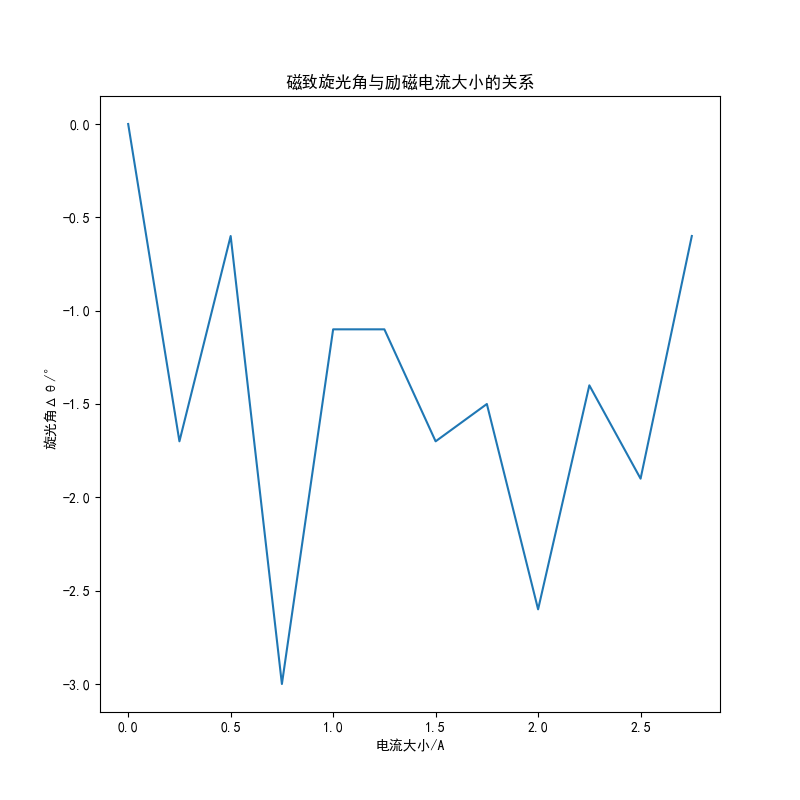
\includegraphics[width=0.5\textwidth]{./images/lab11/T3_1.png}
    
    \label{fig:magneto_optic_effect1}
\end{figure}

\begin{figure}[H]
    \centering
    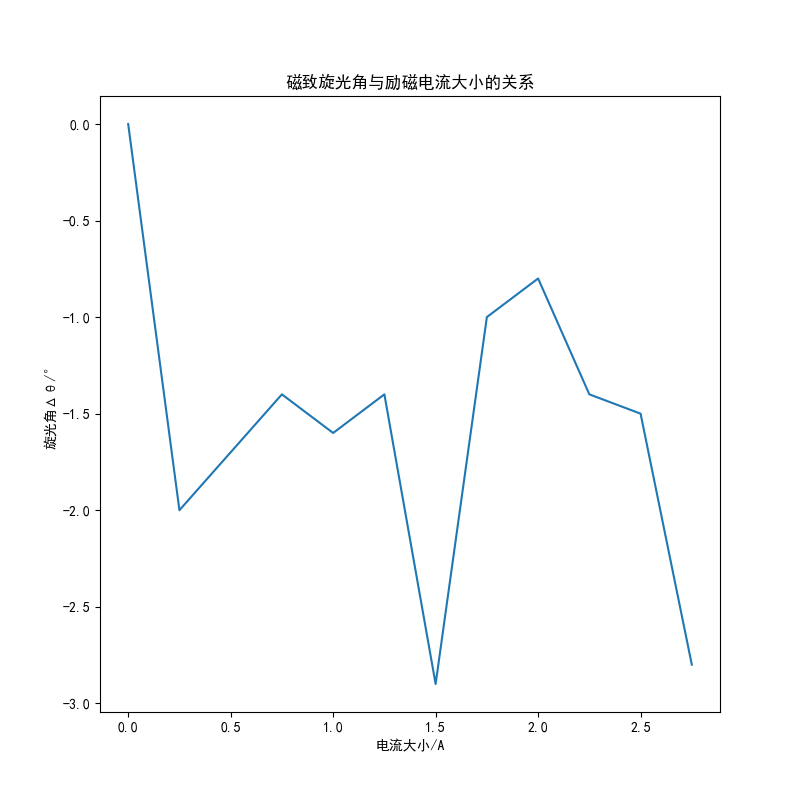
\includegraphics[width=0.5\textwidth]{./images/lab11/T3_2.png}
    
    \label{fig:magneto_optic_effect2}
\end{figure}

\begin{figure}[H]
    \centering
    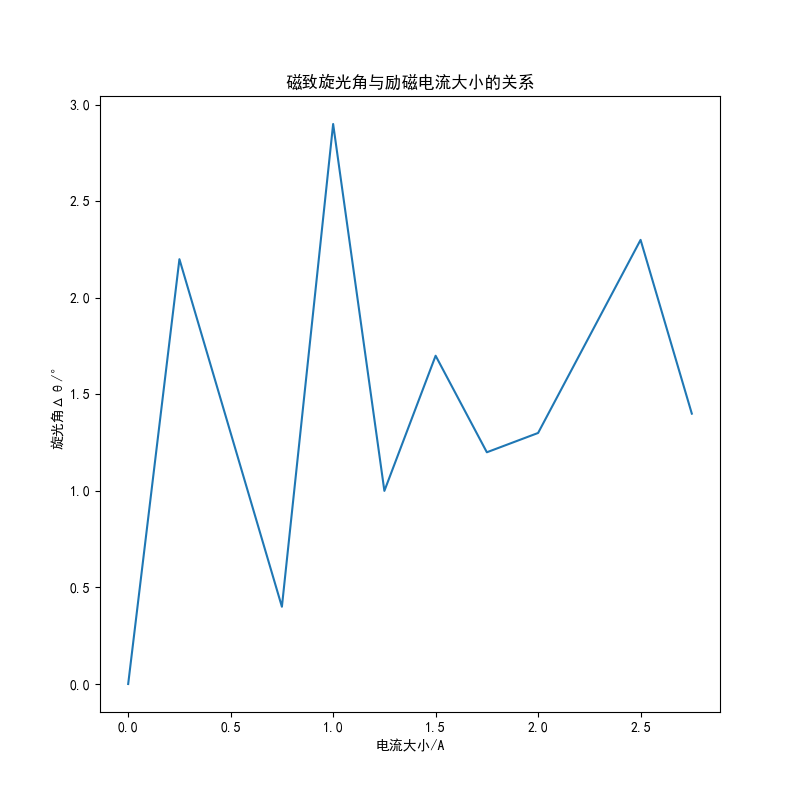
\includegraphics[width=0.5\textwidth]{./images/lab11/T3_3.png}
    
    \label{fig:magneto_optic_effect3}
\end{figure}

实验现象表明,磁致旋光角的方向取决于磁场的方向,而与光束传播的方向无关。大体上旋光角的大小随电流大小的增大而增大。

在音频信号调制实验中,音频信号作为输入,通过实时调节驱动电流来控制磁场的强度,进而改变激光的偏振状态。
光电三极管接收到变化的偏振信号,实现了音频信号的调制。当驱动电流调整到合适的值时,扬声器能够播放出较为清晰的音乐。
\newpage



\section{讨论题}

如图 1 所示,一束偏振光穿过置于线圈之中、长度为 $d$ 的磁光晶体,线圈中通有大小为
$I$ 的电流,电流方向如箭头所示。在磁场作用下,偏振光的偏振方向发生旋转。请根据该结
果,画出图 2 和图 3 中出射光的偏振方向,标出角度值。

\begin{figure}[H]
    \centering
    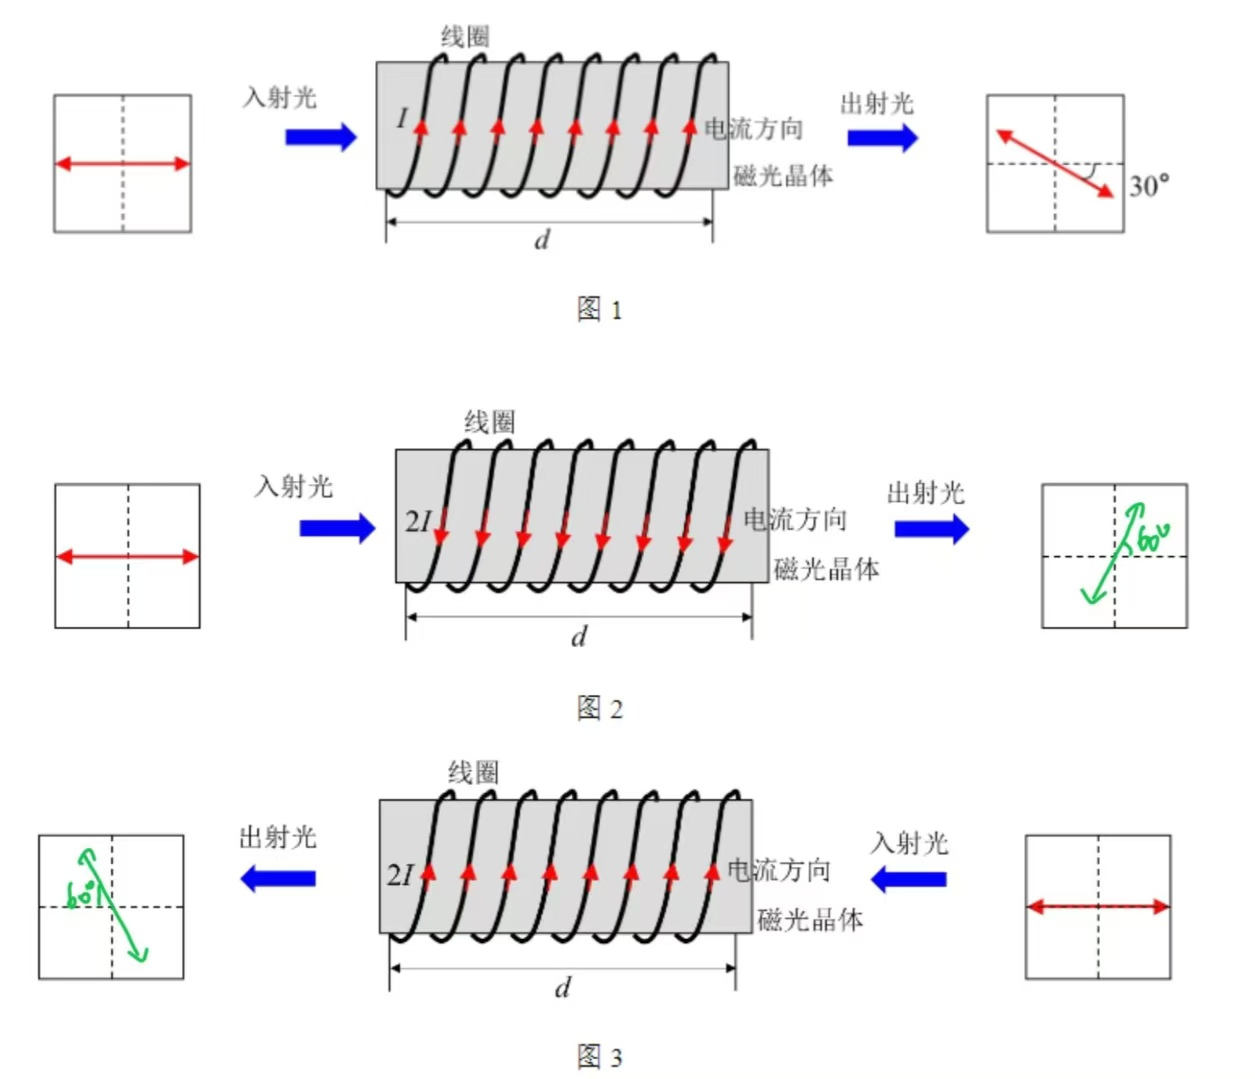
\includegraphics[width=0.8\textwidth]{./images/lab11/T4.jpg}
    
    \label{fig:magneto_optic_effect}
\end{figure}


\end{document}